% TODO: Falar sobre a infraestrutura cloud do front-end

% TODO!: FALAR SOBRE O MULTI-REGION 


\section{Infraestrutura Cloud}
% Explicar sobre o que será abordado nesse capítulo

Neste capítulo, será apresentada a infraestrutura em nuvem utilizada para hospedar a plataforma Codeboard. Serão abordados os serviços de computação, banco de dados, controle de acesso, segurança, balanceamento de carga, escalabilidade, monitoramento, logs, gestão de incidentes, recuperação de desastres, entre outros. 

A infraestrutura foi projetada para ser altamente disponível, com redundância em todas as camadas, de modo que a plataforma Codeboard possa suportar um grande número de usuários simultâneos sem interrupções. Além disso, a infraestrutura foi projetada para ser escalável, de modo que possa crescer ou diminuir de acordo com a demanda, sem a necessidade de intervenção manual.

\subsection{Visão Geral da Arquitetura em Nuvem}

Para garantir a alta disponibilidade e escalabilidade da plataforma Codeboard, a infraestrutura em nuvem do backend foi projetada para seguir o modelo \emph{Multi-Region Active-Active}\ref{multi-region-active-active}, onde a aplicação é distribuída em várias regiões geográficas, de modo que, em caso de falha em uma região, o tráfego seja automaticamente redirecionado para outra região. A arquitetura em nuvem da plataforma Codeboard é composta por várias camadas, cada uma com um conjunto específico de serviços e funcionalidades. A Figura \ref{fig:cloud-architecture} demonstra a visão geral da arquitetura em nuvem da plataforma Codeboard. 

\begin{figure}[H]
    \centering
    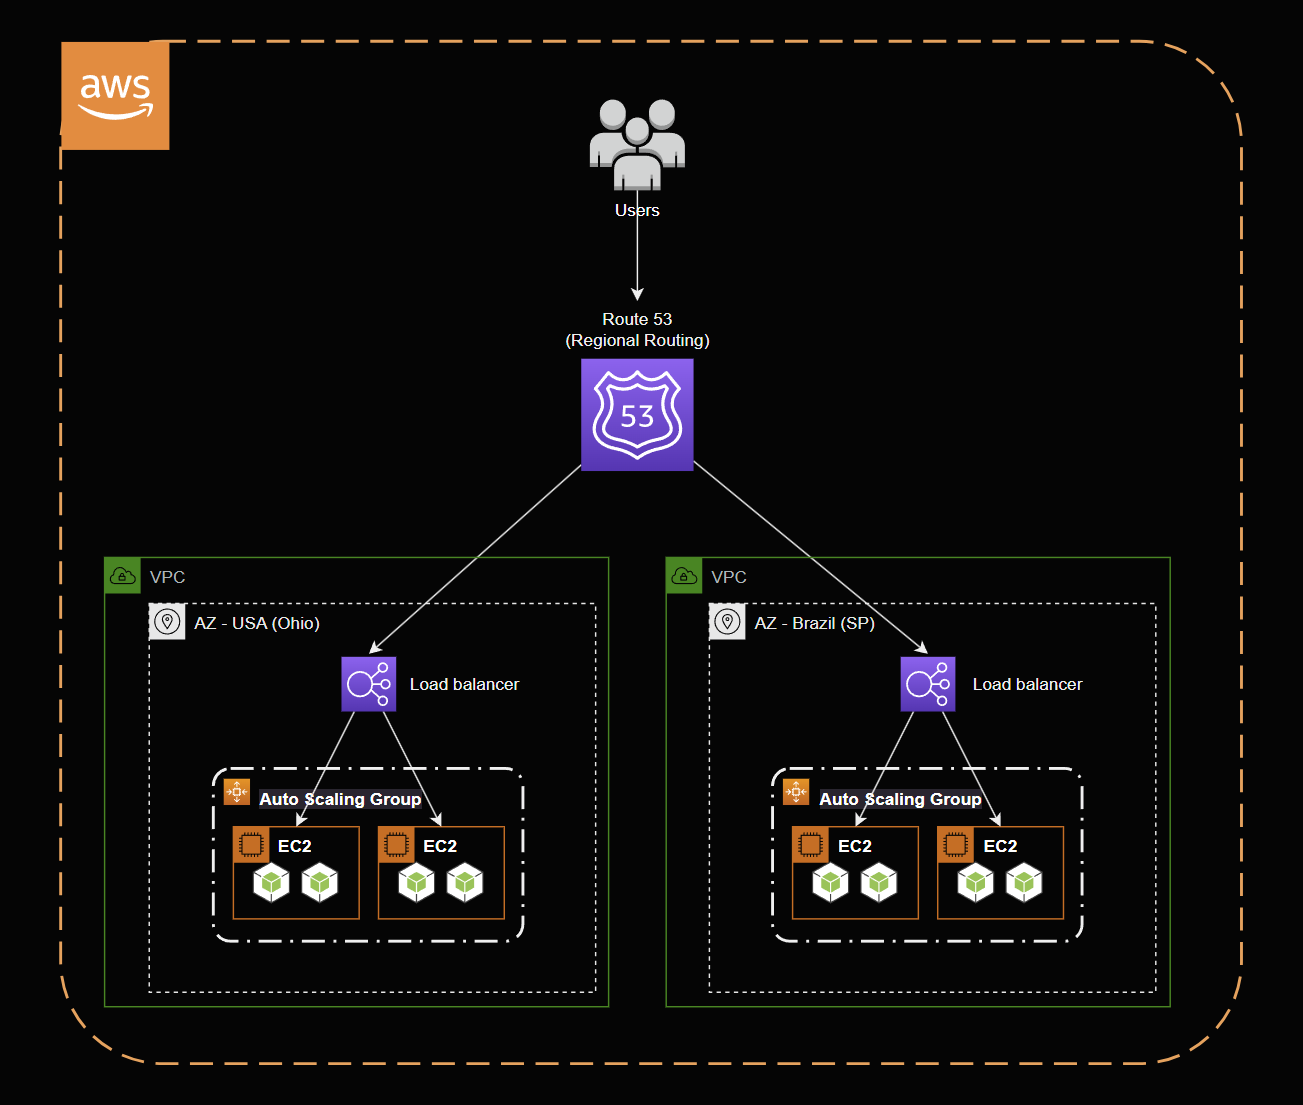
\includegraphics[width=\textwidth]{drawio/cloud-architecture.png}
    \caption{Visão Geral da Arquitetura em Nuvem}
    \label{fig:cloud-architecture}
\end{figure}


\subsubsection{Provedor de Serviços Cloud}
% Por que usar AWS ao invés de Azure ou Google Cloud?
% Benefícios de usar AWS (free-tier, escalabilidade, familiaridade etc)

A plataforma Codeboard foi hospedada na Amazon Web Services (AWS), um dos principais provedores de serviços em nuvem do mercado. A escolha da AWS foi baseada em vários fatores, como a ampla gama de serviços oferecidos, a escalabilidade e a confiabilidade da plataforma, a presença global de data centers, a familiaridade com a AWS, entre outros. A AWS oferece uma variedade de serviços de computação, armazenamento, banco de dados, rede, segurança, monitoramento, entre outros, que são essenciais para a operação da plataforma Codeboard. Além disso, a AWS possui uma vasta rede de data centers em todo o mundo, o que permite a distribuição da aplicação em várias regiões geográficas para garantir alta disponibilidade e baixa latência para os usuários. O \emph{free tier} da AWS também foi um fator importante na escolha da plataforma, pois permite que a plataforma Codeboard seja iniciada sem custos significativos durante o desenvolvimento e testes iniciais.


\subsubsection{Planejamento de Infraestrutura}
% Como a infraestrutura foi planejada?
% Qual é a necessidade da plataforma Codeboard?
% Quais serviços foram escolhidos e por quê?

O planejamento da infraestrutura da plataforma se iniciou com o levantamento dos requisitos e necessidades da aplicação, sendo eles os seguintes:

\begin{itemize}
    \item \textbf{Baixa latência}: a plataforma Codeboard, por ser uma aplicação em tempo real, precisa de baixa latência para garantir uma experiência de usuário fluida e responsiva.
    \item \textbf{Alta disponibilidade}: a plataforma Codeboard deve estar disponível 24 horas por dia, 7 dias por semana, sem interrupções, mesmo durante atualizações e manutenções.
    \item \textbf{Escalabilidade}: a plataforma Codeboard deve ser capaz de suportar um grande número de usuários simultâneos, crescendo ou diminuindo seus recursos de acordo com a demanda.
    \item \textbf{Resiliência}: a plataforma Codeboard deve ser capaz de se recuperar automaticamente de falhas de hardware ou software, sem afetar a experiência do usuário.
    \item \textbf{Recuperação de desastres}: a plataforma Codeboard deve ser resiliente a falhas e desastres, de modo que a operação seja mantida mesmo em caso de falhas em uma região geográfica do provedor de nuvem.
    \item \textbf{Custo-efetividade}: a infraestrutura da plataforma Codeboard deve ser otimizada para minimizar os custos operacionais, evitando recursos ociosos e desnecessários.
    \item \textbf{Facilidade de gerenciamento}: a infraestrutura da plataforma Codeboard deve ser fácil de gerenciar e manter, sendo implementada com boas práticas de DevOps e automação, como \emph{Infra-as-Code} (IaC) e \emph{Continuous Integration/Continuous Deployment} (CI/CD).
    \item \textbf{Segurança}: a plataforma Codeboard deve ser segura e protegida contra ameaças e ataques cibernéticos.
    \item \textbf{Conformidade}: a plataforma Codeboard deve estar em conformidade com as regulamentações e padrões de segurança da indústria.
    \item \textbf{Monitoramento}: a plataforma Codeboard deve possuir métricas e logs para monitorar o desempenho e a integridade da aplicação. 
\end{itemize}

Com base nos requisitos e necessidades da plataforma Codeboard, foram escolhidos os seguintes serviços da AWS para compor a infraestrutura da aplicação:

\begin{itemize}
    \item Amazon Elastic Compute Cloud (EC2): serviço de computação em nuvem que fornece instâncias virtuais escaláveis e seguras para executar a aplicação.
    \item Amazon Elastic Load Balancing (ELB): serviço de balanceamento de carga que distribui o tráfego entre várias instâncias EC2 para garantir alta disponibilidade e escalabilidade.
    \item AWS Auto Scaling: serviço de escalabilidade automática que ajusta automaticamente a capacidade das instâncias EC2 com base na demanda.
    % \item Amazon DocumentDB: serviço de banco de dados NoSQL que fornece instâncias gerenciadas de bancos de dados MongoDB.
    % \item Amazon ElastiCache: serviço de cache em memória que fornece instâncias gerenciadas de Redis.
    \item Amazon Virtual Private Cloud (VPC): serviço de rede virtual que permite a criação de sub-redes privadas, gateways de internet, regras de firewall, entre outros.
    \item Amazon Route 53: serviço de DNS que permite a configuração de registros de DNS, balanceamento de carga, failover, entre outros.
    \item Amazon CloudWatch: serviço de monitoramento e observabilidade que fornece métricas, logs e alarmes para monitorar a saúde e o desempenho da aplicação.
    \item AWS Identity and Access Management (IAM): serviço de controle de acesso e segurança que permite a criação de usuários, grupos, políticas, papéis, entre outros.
    \item AWS Certificate Manager (ACM): serviço de gerenciamento de certificados SSL/TLS que permite a criação, renovação e implantação de certificados SSL/TLS.
\end{itemize}

\subsection{Infraestrutura de Computação}

Tendo em vista que será utilizado o modelo \emph{Multi-Region Active-Active}, a infraestrutura de computação da plataforma Codeboard foi projetada para ser distribuída em várias regiões geográficas da AWS, de modo que, em caso de falha em uma região, o tráfego seja automaticamente redirecionado para outra região. A infraestrutura de computação é composta por instâncias EC2, balanceamento de carga, escalabilidade automática, controle de acesso e segurança, monitoramento, logs, gestão de incidentes, recuperação de desastres, entre outros.

\subsubsection{Máquinas Virtuais}
% Quais instâncias foram escolhidas e por quê? (t3.micro, free-tier, 2 cores etc)
% Como as instâncias foram configuradas? (Ubuntu, NGINX, firewall, etc)

Para hospedar a aplicação da plataforma Codeboard, foram escolhidas instâncias EC2 do tipo \emph{t3.micro}, ela é uma instancia ideal para o estudo de caso pelos seguintes motivos: 

\begin{itemize}
    \item \textbf{Custo}: as instâncias \emph{t3.micro} são parte do \emph{free tier} da AWS, o que significa que elas são gratuitas durante os primeiros 12 meses de uso.
    \item \textbf{Performance Escalável}: as instâncias \emph{t3.micro} possuem a capacidade de burst, o que significa que elas podem fornecer mais recursos de CPU temporariamente quando necessário, sem custos adicionais.
    \item \textbf{2 vCPUs}: as instâncias \emph{t3.micro} possuem 2 vCPUs, que é o mínimo recomendado para a aplicação da plataforma Codeboard, que será executada em um \emph{cluster} de processos, onde cada processo é uma aplicação Node.js que é responsável pelo backend.
    \item \textbf{1 GB de memória RAM}: as instâncias \emph{t3.micro} possuem 1 GB de memória RAM, que é mais que suficiente para a aplicação da plataforma Codeboard, que é leve e não requer muitos recursos de memória devido a sua natureza de ser um intermediário de mensagens em tempo real.
    \item \textbf{Armazenamento em disco SSD}: as instâncias \emph{t3.micro} possuem armazenamento em disco SSD, que é mais rápido e confiável do que o armazenamento em disco magnético. Por mais que a aplicação da plataforma Codeboard não faça uso intensivo de disco, o armazenamento em disco SSD acaba sendo um benefício adicional.
\end{itemize}

As instâncias EC2 foram configuradas com o sistema operacional \emph{Ubuntu 20.04 LTS}, o servidor web \emph{NGINX}, o gerenciador de processos \emph{PM2} e entre outras ferramentas. O Ubuntu 20.04 LTS foi escolhido por ser uma distribuição Linux estável e de longo prazo, com suporte a atualizações de segurança de longo prazo. O NGINX foi escolhido como servidor web reverso para redirecionar o tráfego HTTPS para o processo Node.js, que é responsável pela aplicação da plataforma Codeboard. O PM2 foi escolhido como gerenciador de processos para manter os processos Node.js em execução e reiniciá-los automaticamente em caso de falha. 

\subsubsection{Balanceamento de Carga entre Processos e Tolerancia à Falhas de Processos}

Como a aplicação da plataforma Codeboard é executada em um \emph{cluster} de processos, foi necessário implementar um balanceamento de carga entre os processos para distribuir o tráfego de entrada de forma equilibrada e eficiente. Para isso, o PM2 foi configurado com o modo \emph{cluster}, que cria vários processos Node.js que compartilham o mesmo \emph{socket} de rede, permitindo que o NGINX distribua o tráfego entre eles. O NGINX foi configurado com o módulo \emph{proxy\_pass} para redirecionar o tráfego HTTPS para o processo Node.js, que é responsável pela aplicação da plataforma Codeboard. 

O algorithm de balanceamento de carga do NGINX foi configurado como \emph{Round Robin}, que distribui o tráfego de entrada de forma equilibrada entre os processos do \emph{cluster}, garantindo que todos os processos recebam uma quantidade igual de requisições. A Figura \ref{fig:pm2-load-balancing} demonstra o balanceamento de carga com Round Robin entre os processos Node.js.

% TODO: Adicionar imagem do balanceamento de carga entre processos

O balanceamento de carga entre os processos garante que os recursos de CPU e memória sejam utilizados de forma eficiente, distribuindo a carga de trabalho de forma equilibrada entre os vCPUs disponíveis nas instâncias EC2. Além disso, o balanceamento de carga entre os processos aumenta a disponibilidade e a confiabilidade da aplicação, pois, em caso de falha em um processo, o tráfego é automaticamente redirecionado para outro processo, sem interrupções para os usuários.

Para garantir a tolerância à falhas e a alta disponibilidade da aplicação, foram configurados, no PM2, mecanismos de monitoramento e recuperação de falhas, que monitora os processos Node.js e os reinicia automaticamente em caso de falha. A Figura \ref{fig:pm2-fault-tolerance} demonstra como o PM2 monitora os processos Node.js e os reinicia em caso de falha.

% TODO: Adicionar imagem da tolerância à falhas

\subsubsection{Controle de Acesso e Segurança}

Para garantir a segurança da infraestrutura de computação da plataforma Codeboard, foram implementadas várias políticas de segurança, como:

\begin{itemize}
    \item \textbf{AWS Identity and Access Management (IAM)}: foram criados políticas e papéis no IAM para controlar o acesso aos recursos da AWS. Utilizando permissões restritas para as instâncias EC2, permitindo apenas as ações necessárias para a execução da aplicação, de acordo com o princípio do menor privilégio. % TODO: Possível Referência?
    \item \textbf{Firewall}: foram configuradas regras de firewall no \emph{Security Group} da VPC para restringir o tráfego de entrada e saída para as instâncias EC2. Foram permitidas apenas as portas necessárias para o funcionamento da aplicação. Com exceção da porta 80 (HTTP) e a porta 22 (SSH) que é aberta apenas para os endereços IP autorizados, todas as outras portas entrantes são bloqueadas.
    \item \textbf{Chaves SSH}: foram criadas chaves SSH para autenticação de usuários durante o acesso remoto às instâncias EC2. 
\end{itemize}

As instâncias EC2 não são acessadas diretamente, elas recebem o tráfego de entrada através do balanceamento de carga do ELB, que distribui o tráfego de forma equilibrada entre as instâncias EC2. Nele foi configurado um certificado SSL para garantir a criptografia do tráfego entre o cliente e o servidor, garantindo a segurança dos dados em trânsito. O ELB também foi configurado com um \emph{Security Group} para restringir o tráfego de entrada, permitindo apenas a porta 443 (HTTPS) e para o tráfego de entrada.

\subsubsection{Balanceamento de Carga entre Máquinas Virtuais}

A infraestrutura de computação da plataforma Codeboard foi projetada para ser altamente distribuída e redundante, de modo que o tráfego seja distribuído entre várias instâncias EC2 em diferentes regiões geográficas. Para isso, foi configurado um balanceamento de carga entre as instâncias EC2, utilizando o serviço AWS Elastic Load Balancing (ELB). O ELB distribui o tráfego de entrada de forma equilibrada entre as instâncias EC2, garantindo alta disponibilidade e escalabilidade da aplicação.

Existem vários tipos de ELB disponíveis na AWS, como o Application Load Balancer (ALB), Network Load Balancer (NLB) e Classic Load Balancer (CLB). Para a plataforma Codeboard, foi escolhido o Application Load Balancer (ALB), que é um balanceador de carga de camada 7 que opera no nível de aplicação, permitindo o roteamento de tráfego com base em regras de conteúdo, como URL, cabeçalhos HTTP, métodos HTTP, entre outros. O ALB foi configurado com um certificado SSL para garantir a segurança do tráfego HTTPS entre o cliente e o servidor.

O algoritmo de balanceamento de carga utilizado pelo ELB foi configurado como \emph{Round Robin}, que distribui o tráfego de entrada de forma equilibrada entre as instâncias EC2, garantindo que todas as instâncias recebam uma quantidade igual de requisições. 

% TODO?: Voltar no capítulo 3 para explicar a importância do Health Check? Testar se a conexão com o banco de dados está funcionando, se a aplicação está respondendo, etc.
Para garantir que apenas instâncias saudáveis recebam tráfego, foram configurados \emph{Health Checks} para monitorar a saúde das instâncias EC2. Health Checks são verificações periódicas que o ELB realiza em cada instância para garantir que ela esteja saudável e pronta para receber tráfego. Uma rota de Health Check foi implementada na aplicação da plataforma Codeboard, de modo que o ELB possa verificar se a aplicação está respondendo corretamente. Se uma instância falhar no Health Check, o ELB a marca como indisponível e redireciona o tráfego para outras instâncias saudáveis. A Figura \ref{fig:elb-health-check} demonstra como funciona o Health Check do ELB.

% TODO: Adicionar imagem do Health Check do ELB, talvez um diagrama de sequência? Importante para explicar o funcionamento do Health Check, 3 tentativas, intervalo de tempo, etc.

\subsubsection{Escalabilidade Horizontal e Recuperação Automática de Falhas}

% Por que usar escalabilidade horizontal ao invés de vertical? (disponibilidade)
Como um dos requisitos da plataforma Codeboard é a alta disponibilidade, a infraestrutura de computação foi projetada para ser escalável horizontalmente, de modo que a aplicação possa aumentar ou diminuir seus recursos acordo com a demanda, sem a necessidade de intervenção manual. Para isso, foi configurado o serviço AWS Auto Scaling, que ajusta automaticamente a quantidade de instâncias EC2 com base na demanda.

O Auto Scaling foi implementado com um Auto Scaling Group (ASG) que monitora a utilização da CPU das instâncias EC2 e ajusta a quantidade de instâncias com base em uma política de escalabilidade. Foram definidos gatilhos de escalabilidade para aumentar ou diminuir a quantidade de instâncias com base na utilização da CPU. Se a utilização da CPU de uma instância ultrapassar um determinado limite por um período de tempo, o ASG adiciona uma nova instância para distribuir a carga de trabalho. Se a utilização da CPU de uma instância cair abaixo de um determinado limite por um período de tempo, o ASG remove a instância para economizar custos. Além disso, ele foi configurado com um número mínimo e máximo de instâncias para garantir que os custos sejam controlados e um nível mínimo de capacidade seja mantido. 

Os valores de configuração dos gatilhos de escabilidade foram decididos arbitrariamente, com base em testes e observações do comportamento da aplicação. Foi definido um limite de 70\% de utilização da CPU para adicionar uma nova instância e um limite de 30\% de utilização da CPU para remover uma instância. Além disso, foi definido um número mínimo de 1 instância e um número máximo de 5 instâncias em execução. Esses valores podem ser ajustados conforme necessário, com base em previsões de tráfego, sazonalidade, eventos especiais, entre outros.

% Como funciona a tolerância à falhas? (Health Check, Auto Scaling, etc)

O Auto Scaling também foi configurado com um mecanismo de recuperação automática de falhas, que monitora a saúde das instâncias EC2 e as substitui em caso de falha. Se uma instância falhar no Health Check e for marcada como indisponível pelo ELB, o Auto Scaling a substitui por uma nova instância saudável, garantindo que a aplicação permaneça disponível e resiliente a falhas. A combinação do Auto Scaling com o ELB e o PM2 garante que a aplicação da plataforma Codeboard seja altamente disponível, escalável e resiliente a falhas. A Figura \ref{fig:auto-scaling-fault-tolerance} demonstra como funciona a recuperação automática de falhas com o Auto Scaling.

% TODO: Adicionar imagem da recuperação automática de falhas com o Auto Scaling, talvez um diagrama de sequência? Importante para explicar o funcionamento da recuperação automática de falhas, substituição de instâncias, etc.

\subsection{Banco de Dados MongoDB}

\subsubsection{Provedor de Banco de Dados}
% Onde o banco de dados está hospedado?
% Benefícios de usar MongoDB Atlas ao invés de um banco de dados local

\subsubsection{Escalabilidade Vertical Automática}
% Por que usar escalabilidade vertical ao invés de horizontal? (custo, complexidade, etc)
% Como a escalabilidade vertical foi configurada?
% Quais são os gatilhos para aumentar ou diminuir a capacidade do banco de dados?

\subsubsection{Backup e Recuperação de Dados}
% Como os backups são feitos?
% Como os backups são armazenados?

\subsubsection{Controle de Acesso e Segurança}
% Como o controle de acesso foi configurado?
% Quais são as políticas de segurança?

\subsection{Banco de dados Redis}

\subsubsection{Provedor de Banco de Dados}
% Onde o banco de dados está hospedado?
% Benefícios de usar Redis ao invés de um banco de dados local

\subsubsection{Sharding e Replicação}
% Por que usar escalabilidade horizontal ao invés de vertical? (disponibilidade, latência, etc)
% Como o sharding foi configurado?
% Como a replicação foi configurada?

\subsubsection{Controle de Acesso e Segurança}
% Como o controle de acesso foi configurado?
% Quais são as políticas de segurança?

\subsection{Estrutura de Subnets e Controle de Acesso à Rede}

\subsection{Controle de Tráfego}

\subsubsection{Configurações de DNS}
% Como o DNS é configurado? Para onde ele aponta?
% Como o tráfego é controlado? Como é feito o balanceamento de carga?

\subsubsection{Balanceamento de Carga entre Regiões}

\subsubsection{Configurações de SSL}

\subsection{Distribuição de Conteúdo (CDN)}
% Por que usar Vercel ao invés de outro?
% Vercel é um PaaS, por que escolher um PaaS ao invés de um IaaS?

\subsubsection{Plataforma de Distribuição de Conteúdo}
% Por que usar Vercel ao invés de outro?
% O que é CDN e por que é importante?
% Benefícios de usar CDN

\subsubsection{Configuração da CDN}
% Como a CDN foi configurada?

\subsection{Monitoramento, Logs e Gestão de Incidentes}
% Como o monitoramento é feito?

\subsubsection{Monitoramento da Aplicação}
% Como o monitoramento da aplicação é feito?
% Quais métricas são monitoradas?

\subsubsection{Monitoramento de Recursos da Nuvem}
% Como o monitoramento de recursos da nuvem é feito?
% Quais métricas são monitoradas?

\subsubsection{Monitoramento de Logs}

\subsubsection{Gestão de Incidentes}
% Como os incidentes são gerenciados?
% Quais alertas são configurados?

\subsection{Recuperação de Desastres}
% Como a recuperação de desastres é feita?
% Quais são os planos de contingência?
% Como é feito o backup e a recuperação de dados?

% \subsection{Considerações de Latência e Custo}

